\documentclass[12pt, letterpaper]{article}
  \usepackage[utf8]{inputenc}
  \usepackage[left = 2.5cm, right = 2.5cm, top = 3cm, bottom = 3cm]{geometry}
  \usepackage[T1]{fontenc}
  \usepackage{graphicx}
  \graphicspath{{images/}}

  \author{Hernández Ferreiro Enrique Ehécatl \\
          López Soto Ramses Antonio}

        \title{Práctica 4: Unidad aritmetico-lógica (ALU) \\
                {\small Organización y Arquitectura de Computadoras}}
                \date{6 de marzo de 2019}

  \begin{document}
    \maketitle

    \section{Introducción}

      \hspace{.5cm}
      Las computadoras en la actualidad están conformadas por múltiples núcleos
      y, a su vez, también incorporan varias unidades aritmético-lógicas, lo que
       conocemos como \textit{ALU}.\vspace{.3cm}

      En el año de 1945 el mátemático \textbf{John Von Neumann} a través de EDVAC
      proporcionó la idea de la ALU argumentando que era un requisito muy
      importante para que una computadora pudiera ser capaz de efectuar las
      operaciones matemáticas básicas.\vspace{.3cm}

      La ALU es la encargada de realizar operaciones entre distintos tipos de
      datos entre las cuales se encuentran:

        \begin{itemize}
          \item Suma
          \item Resta (complemento a 2)
          \item Operaciones lógicas como OR y AND
        \end{itemize}

      La ALU se encuentra contenida tanto en circuitos básicos como un reloj o
      una calculadora como en citcuitos mucho más complejos como los microchips
      en las computadoras de los últimos años.\vspace{.3cm}

    \section{Desarrollo}

      \hspace{.5cm}
      Para el desarrollo de esta práctica se utilizo el software \textit{Logisim}.\vspace{.3cm}

      Los circuitos uitlizados para el desarrollo de la ALU se presentará a
      continuacion, se utilizaron componentes ya predefinidos y otros fueron
      implementandos.\vspace{.3cm}

      \subsection*{NOT}

        \begin{center}
          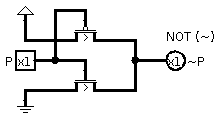
\includegraphics[scale=0.4]{not.png}
        \end{center}

      \subsection*{OR}

        \begin{center}
          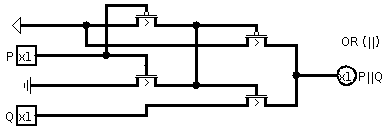
\includegraphics[scale=0.4]{or.png}
        \end{center}

      \subsection*{XOR}

        \begin{center}
          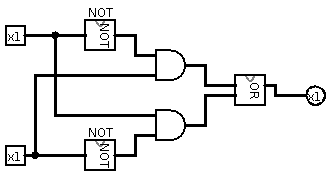
\includegraphics[scale=0.4]{xor.png}
        \end{center}

        \subsection*{Comparador}
          \begin{center}
            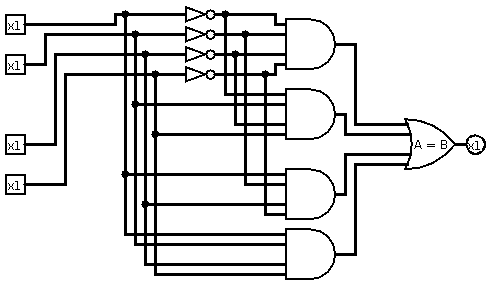
\includegraphics[scale=0.4]{comp.png}
          \end{center}

        A partir de este punto todo lo anterior fue usado para la implementación
        de la simulación de una ALU en Logisim.

      \subsection*{Sumador completo \textit{full adder}}

        \begin{center}
          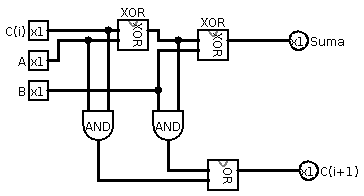
\includegraphics[scale=0.4]{sumador.png}
        \end{center}

      \subsection*{ALU 1 bit}

        \begin{center}
          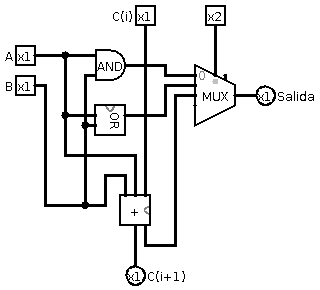
\includegraphics[scale=0.6]{alu_1.png}
        \end{center}

      \subsection*{ALU 8 bits}

        \begin{center}
          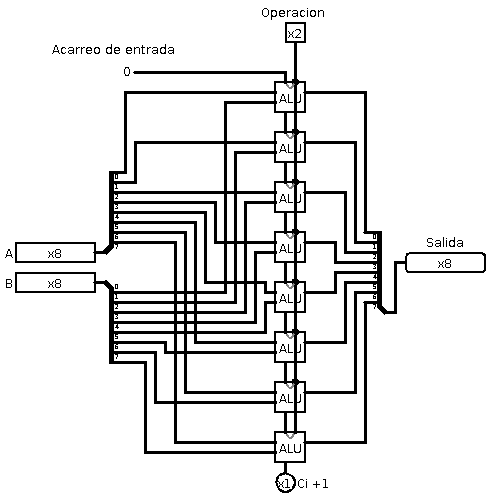
\includegraphics[scale=0.6]{alu_8.png}
        \end{center}

      \subsection*{ALU 1 bit (resta)}

        \begin{center}
          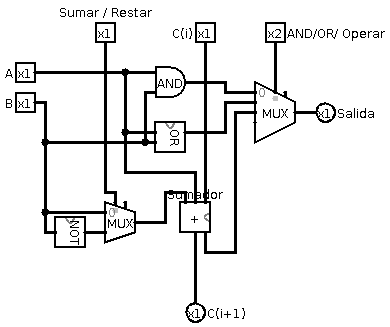
\includegraphics[scale=0.6]{alu_res.png}
        \end{center}

      \subsection*{ALU 8 bits (igualdad)}

        \begin{center}
          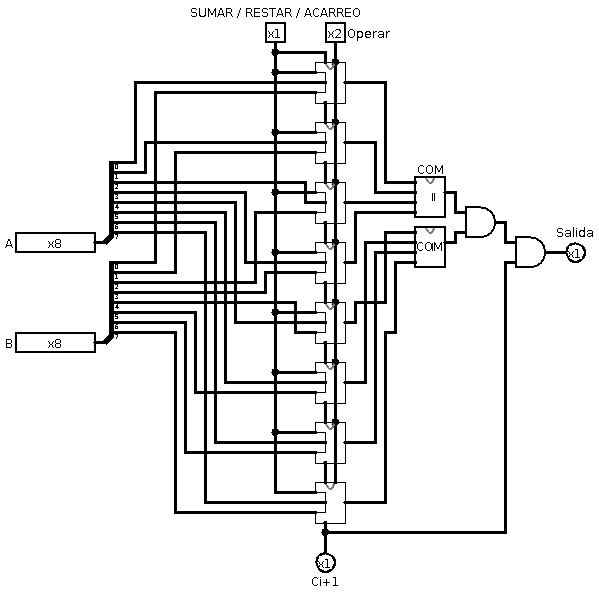
\includegraphics[scale=0.5]{alu_eq.png}
        \end{center}

      \subsection*{ALU NOR}

        \begin{center}
          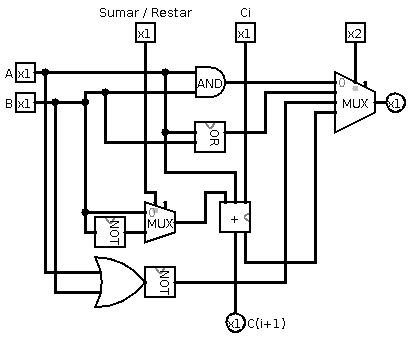
\includegraphics[scale=0.6]{alu_nor.png}
        \end{center}

      \subsection*{ALU final}

        \begin{center}
          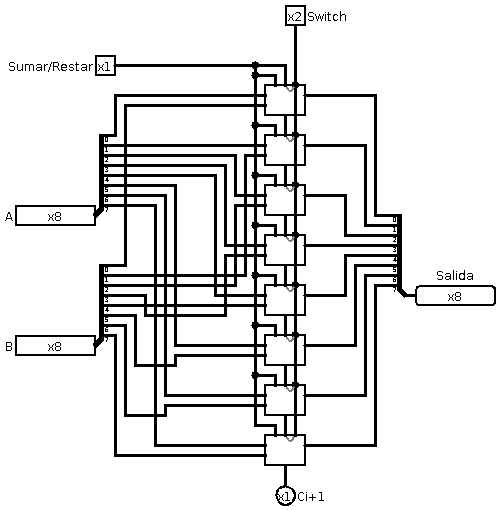
\includegraphics[scale=0.6]{alu_f.png}
        \end{center}

    \section{Conclusión}

      \hspace{.5cm}
      En resumen, la ALU es uno de los componentes dentro del CPU, pues gracias
      a ella es posible la realización de las operaciones matemáticas elementales
      y de las operaciones lógicas, esto la hace muy importante para la
      computación ya que en eso se basan los algoritmos.\\
      
      \subsection{Preguntas}

        \begin{itemize}
          \item[1.] ¿Qué operaciones aritméticas y lógicas  son básicas para un
                    procesador? \vspace{.2cm}

                    \textbf{R.} Las operaciones básicas para un procesador son:
                                la suma aritmética, la resta aritmética
                                (complemento a 2) y logicas como: AND, OR y NOT.
                                Pues con estás operaciones es posible realizar lo
                                necesario para que una computadora funcione.

          \item[2.] El diseño utilizado para realizar la adición resulta ser
                    ineficiente, ¿por qué? ¿Qué tipo de sumador resulta ser más
                    eficiente? \vspace{.2cm}

                    \textbf{R.} Resulta ser ineficiente pues recibe tres bits de
                                entrada, dos de ellos son los bits que se desean
                                sumar y el restante es el acarreo que proviene de
                                de la operación anterior menos significativa; y
                                además, tiene dos salidas: el resultado y el
                                desbordamiento.\\
                                Un sumador más eficiente podrían ser los llamados
                                \textit{sumadores con acarreo anticipado}. O
                                también dividir el sumador en varias partes para
                                así optimizar el tiempo de cálculo.

          \item[3.] Bajo este diseño, en la ALU se calculan todas las operaciones
                    de forma simultánea pero sólo se entrega un resultado, ¿se
                    realiza trabajo inútil? ¿Toma tiempo adicional? ¿Cuál es el
                    costo? \vspace{.2cm}

                    \textbf{R.} No. La operación esta determinada por el bit que
                                indicado para que así no se realice trabajo innecesario.
                                Aunque si tom a un poco más de tiempo a una ALU
                                que sólo se dedique a realizar una sola operación.

          \item[4.] ¿Cuántas operaciones más podemos agregar al diseño de la ALU?
                    ¿Qué tendríamos que modificar para realizar más operaciones? \vspace{.2cm}

                    \textbf{R.} A la ALU se le puede agregar la multiplicación y
                                la división entera; sólo bastaría con implementar
                                un multiplicador y un divisor y agregarlo en la
                                ALU modificando algunas conexiones con los bits
                                de entrada y los acarreos.
        \end{itemize}

  \end{document}
